% -*- mode: LaTeX; coding: utf-8; -*-

\chapter{Analyysi}

Tässä luvussa käydään vaiheittain läpi yhden valitun palvelun analysointi sekä esitetään perustelut, joiden pohjalta tehtyihin ratkaisuihin päädyttiin. 
Luvussa myös esitellään analysoinnista saatuja tuloksia, sekä pohditaan näihin johtaneita syitä. Lopuksi vielä esitetään jatkotutkimuksen kannalta 
tärkeitä kehitysideoita, joita syntyi tutkimuksen aikana. 
 
\section{Tutkimuksen toteutus}

Saamamme materiaali koostui neljästä eri Web-palvelusta, joista analyysiin valitsimme yhden. Muista palveluista saadut lokitiedostot käsiteltiin
myös valmiiksi, mutta koska lokitietoja oli määrällisesti niin paljon, päädyimme tarkastelemaan tarkemmin vain yhtä. Valitsemastamme palvelusta
analysoimme myös vain viikon mittaisen jakson. Tähän ratkaisuun päädyttiin sen takia, että analysoitavaa dataa oli kerätty noin puolen vuoden ajalta,
joten jo yhden palvelun osalta koko datan läpikäymiseen olisi mennyt kohtuuttomasti aikaa. Diffuusikuvausten opetusmateriaalin laskemiseen voidaan
myös käyttää korkeintaan noin 5000 yksittäistä pistettä 2000 pisteen ollessa laskennallisesti vielä tehokasta, koska algoritmin aikavaativuus kasvaa
eksponentiaalisesti verrattaessa opetusmateriaalin kokoon. 
 
Esikäsittelyvaiheessa HTTP-kyselyt jaetaan palvelun resurssien mukaan omiin tiedostoihin, joissa ne ovat CVS-formaatissa kuvan ??? mukaisesti. 
Resursseihin kohdistuvat kyselyt vaihtelevat suuresti sen mukaan, kuinka käytetty mikäkin resurssi on. Perinteisen Web-sivuston tapauksessa tähän
vaikuttavat esimerkiksi resurssia käyttävän palvelun käyttöaste ja se, käytetäänkö samaa resurssia useamman sivun osana. 

Analyysissä käyttämämme viikon pituinen jakso sisälsi yhteensä 913 eri resurssia ja näihin kohdistuvat kyselymäärät vaihtelivat muutamasta kappaleesta
aina kymmeniin tuhansiin. Näistä suodatimme pois sellaiset resurssit, joihin kohdistui alle 100 kyselyä ja joiden GET-parametreistä muodostettujen
erilaisten n-grammien määrä oli alle kymmenen. Suodatuksen jälkeen analysoitavaksi jäi 36 resurssia. Käyttämillämme suodatusrajoilla ei ole tekemistä 
itse esikäsittelijän kanssa, vaan suodatusrajat on käyttäjän säädettävissä tiedostosta \texttt{src/InterestingParameters.hs}.
    
Käytetyimmissä resursseissa HTTP-kyselyitä oli kymmeniä tuhansia, joten jokaisesta resurssista ei pystytty suoraan tekemään diffuusiokuvausta johtuen
menetelmän rajoituksista. Ongelma ratkaistiin valitsemalla satunnaisotannalla ilman takaisinpanoa 2000 HTTP-kyselyä niistä resursseista, joissa oli 
kyselyitä yli tämän määrän. Näin ollen jokaisesta resurssista muodostettiin lopulta tiedosto, jossa oli korkeintaan 2000 HTTP-kyselyä.

Analysoitavan palvelun eri resurssit on kuvattu graafissa \ref{service_resources}. Kuvassa vaaka-akselina on käytetty N-grammien lukumäärää ja 
pystyakselina GET-parametrien lukumäärää. Resursseista valitsimme kuusi tarkempaan tarkasteluun, ja ne on merkitty kuvaajaan niiden resurssinumerolla. 
Resurssit pyrimme valitsemaan siten, että jokaisesta ryppäästä on valittu yksi.

\begin{figure}[ht]
\centering
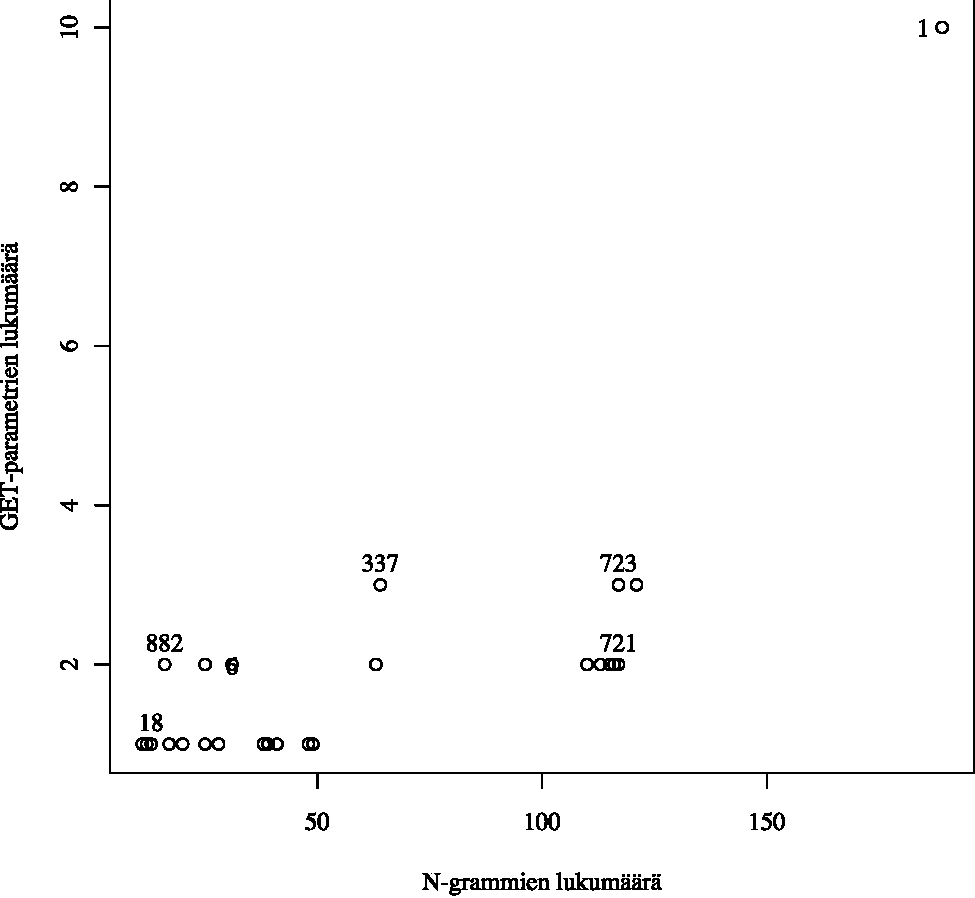
\includegraphics[width=13cm]{pics/service_resources.pdf}
\caption{Palvelun resurssien ominaisuudet}
\label{service_resources}
\end{figure}

\section{Tulokset}




\section{Kehitysideoita}
% Keksi parempi otsikko? :-)

- Reaaliaikaisessa toteutuksessa aikavaativuus ei ole ongelma, koska järjestelmälle opetetaan etukäteen normaali käyttäytyminen, jonka jälkeen
uudet pisteet projisoidaan yksitellen kuvaan. Nyström extension
- Menetelmänt toimivuuden testauksen kannalta tarvittaisiin rajatumpaa materiaalia. Esimerkiksi lyhyempi ajan jakso sellaiselta hetkeltä, jolloin
 tiedetään hyökkäyksen tapahtuneen
- Opetusjakson määrittely

